\subsubsection*{Desarrollo}

\title {Imágenes}

\par Para realizar la experimentación utilizamos la imagen tomo.png provista por la cátedra, con una resolución de 100 x 100 pixeles.
\par La imagen la trabajamos en formato .csv para la entrada con una profundidad de 16 bits y luego de la reconstrucción la guardamos en formato pgm de 8 bits.
\par Para la conversión de la imagen de 16 a 8 bits implementamos una función (to8bits) que identifica los valores de intensidad máximo y mínimo de la imagen a guardar. Al valor mínimo se le asocia el valor de salida 0 y al máximo el valor de salida 255. Los valores de intensidades intermedias se distribuyen de forma proporcional. Este procedimiento permite salvar el inconveniente de que como resultado de la eliminación gaussiana se pueden obtener valores negativos, los cuales no tienen sentido en este contexto ya que representan intensidades que siempre son valores mayores o iguales a cero, o valores mayores al máximo valor permitido para una imagen de 16 bits. Esto es posible porque estamos encontrando una solución aproximada y además estamos trabajando con ruido.

\par En un principio comenzamos utilizando los archivos .csv provistos por la cátedra de 512 x 512 pixeles, con estas imágenes realizamos varias pruebas fallidas que se explican más detalladamente en el apartado Generación de rayos. Debido a diversas dificultades que se nos presentaron con la elección de la estrategia para trazar los rayos, se demoró el inicio de las pruebas y optamos por utilizar imágenes más chicas para poder realizarlas en el tiempo de que disponíamos. Aunque hubiera sido interesante poder trabajar con un conjunto mayor de imágenes.

\title {Discretización} Para discretizar la imagen utilizamos valores divisores de 100. En los tests de granularidad, variamos el tamaño de las celdas tomando los valores 4x4, 5x5, 10x10, 20x20, 25x25 y 50x50 pixeles. Como ya se analizó a medida que se achica el tamaño de las celdas crece el tiempo de procesamiento, lo cual condicionó la elección de los parámetros.

\title {Cálculo de la distancia recorrida por cada rayo} 
Implementamos una función “pasa” que se encarga de identificar por qué pixeles pasa un rayo (los rayos son considerados como rectas en el plano, caracterizados por un punto de origen que llamamos $(x_{0},y_{0})$ y un ángulo $\alpha$ ).

\par Para poder describir esta función adecuadamente imaginamos la imagen ubicada en un eje de coordenadas de modo tal que su vértice inferior izquierdo se encuentre en la coordenada (0,0). Pensamos a la imagen como un subconjunto de puntos del plano.

\par Utilizando la tangente de $\alpha$ (que es la pendiente de la recta asociada al rayo), se busca la intersección con la recta $y=0$ la cual es el punto $(x-y/tangent(\alpha),0)$.  De ahi en mas se utiliza la ecuación de la recta $y=tan(\alpha)*x+y_{0}$, variando el valor de $x$ para calcular los puntos del plano (siempre hablando del plano en un sentido general) por los que pasa la recta. Si el punto hallado pertenece a la imagen se guardan las coordenadas del pixel correspondiente en un vector, para ser usadas posteriormente para el cálculo de distancias y de tiempos.

\par Esta función se usa para calcular el tiempo que le toma a un rayo atravesar al sujerto. Para esp se hace la suma de las intensidades de los pixeles por las que pasa el rayo ya que la intensidad de los mismos la asociamos al tiempo que le toma a un rayo atravesar el mismo.

\par Finalmente se la reutilizará por ultima vez para calcular la cantidad de pixeles en cada celda por las que pasa el rayo. Para hacer esto se calcula para cada pixel por los que pasa el rayo a qué celda pertenece. Para esto es necesario realizar una conversión en las coordenadas, ya que las celdas de la imagen se identifican desde la esquina superior izquierda.

\par Debido a que los rayos pasan solamente por algunas celdas del total (Se puede ver gráficamente que si la grilla es de n celdas, a lo sumo serán $2*n-1$), para la matriz de distancias reutilizamos la estructura de matriz esparza del TP1.

\title{Generación de rayos}

\par Una de las decisiones que tuvimos que tomar fue de qué forma trazar los rayos simulados que íbamos a aplicar a la imagen.

\par En cuanto a la cantidad de rayos, la misma debe ser mayor que $n^{2}$, siendo $n$ la cantidad de celdas de la discretización, ya que con una cantidad menor habría celdas que no son atravesadas por ningún rayo. En ese caso, hay columnas completas de ceros en la matriz de distancias, lo cual se traduce en filas de ceros en la matriz del sistema a resolver que como ya explicamos en la introducción se obtiene como $D^{t}D t = D^{t} v$. Esta situación se corresponde con un sistema con infinitas soluciones.

\par En cuanto a la ubicación de los emisores, inicialmente pensamos en dos opciones que resultaron fallidas:
\begin{enumerate}
\item Trazar rayos horizontales y verticales, formando una cuadrícula.
\item Trazar rayos saliendo de los cuatro vértices de la imagen en distintos direcciones para barrer los $90^{\circ}$ de cada ángulo.
\end{enumerate}

\par En ambos casos, al comenzar la experimentación nos encontramos con dificultades.

\par En el primer caso al realizar la eliminación gaussiana nos encontrábamos con que la matriz tenía filas completas en cero (matriz no inversible).

\par En el segundo caso, si bien se ejecutaban todos los pasos del programa las imágenes reconstruídas no eran reconocibles.

Al realizar un análisis de estos resultados nos dimos cuenta que los rayos trazados de estas formas eran muy similares entre sí y en consecuencia no suministraban información sufuciente para realizar una buena aproximación a la verdadera solución del sistema. Igualmente adjuntamos la implementación en el código a título informativo.

\par Finalmente decidimos trazar rayos desde los cuatro laterales de la imagen. Los emisores se ubican en igual cantidad sobre los lados de la imagen, la ubicación de los emisores se selecciona aleatoriamente en base a una distribución uniforme entre $0$ y $k$, siendo $k$ la cantidad de pixeles por lado de la imagen (es decir suponiendo que la imagen tiene $k*k$ pixeles).

\par De cada uno de estos emisores salen igual cantidad de rayos en ángulos que van entre $0^{\circ}$ a $180^{\circ}$. Los valores de los ángulos también se seleccionan aleatoriamente con distribución uniforme.

\par Si bien este método es aleatorio -con lo que los resultados difícilmente se repitan en corridas sucesivas- utilizando una cantidad suficientemente grande de rayos (como en este caso) por consecuencia de la Ley de los Grandes Números, en general los rayos quedan bien distribuídos a lo largo (y ancho) de la imagen, pudiendo obtener así resultados consistentes en varias corridas.

\par De los tres métodos este fue el que nos dio mejores resultados y el que terminamos eligiendo para realizar la experimentación.

\par Durante la experimentación, para una discretización de imagen de 10 celdas por lado (100 celdas en total), realizamos dos tipos de pruebas:
\begin{enumerate}
\item Sobre la cantidad de emisores, variando entre 20 y 140, aumentando de a 20 ($2*n$ hasta $7*2*n$). Sin aplicar ruido y manteniendo constante la cantidad de rayos por emisor en 100.
\item Sobre la cantidad de rayos por emisor, variando desde 50 hasta 150, aumentando de a 10.  Sin aplicar ruido y manteniendo constante la cantidad de emisores en 100.
\end{enumerate}

\par En la fig. se puede ver el trazado de rayos resultante tomando como base la imagen tomo.png en un tamaño de 25 x 25 pixeles, con una discretización en celdas de 5 x 5 pixeles, usando 25 emisores y 25 rayos por emisor.

\begin{figure}[H] 
\centering
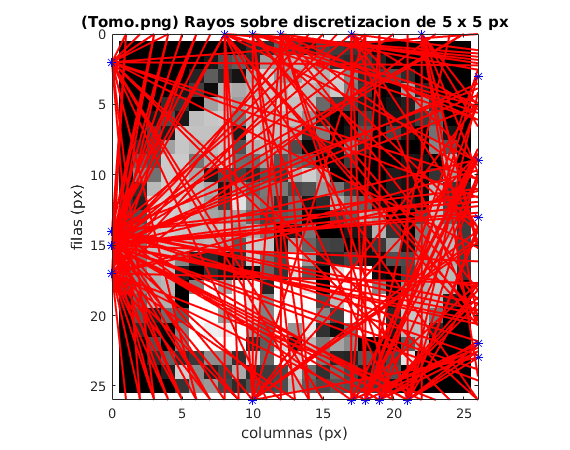
\includegraphics[width=1\textwidth]{img/rayos_tomo25x25px.png}
\caption{Trazado aleatorio de rayos}
\label{fig:rayos aleatorios}
\end{figure}

\title{Cuadrados mínimos} Para resolver el sistema de ecuaciones de cuadrados mínimos utilizamos las ecuaciones normales. Para esto reutilizamos la estructura de matriz esparza y el algoritmo de eliminación gaussiana del TP1, al cual modificamos para utilizar pivoteo de filas.

\par Durante el testeo implementamos la eliminación gaussiana utilizando una matriz completa pero no reportó ningún beneficio en el tiempo de procesamiento por lo cual descartamos la idea.

\title{Ruido} Como explicamos en la introducción utilizamos ruido gaussiano aleatorio multiplicativo sobre el vector de tiempos de recorrida de los rayos de manera que para cada elemento, el resultado luego de aplicar el ruido es $v{1}= v + v * \alpha * x$ con $x$ un valor aleatorio entre 0 y 1 con distribución normal.
Durante la experimentación usamos como parámetro los valores
$x * \alpha$ para $\alpha$ = 0.001 y $x$ tomando valores del conjunto en $\{1,2,3,4,5,6,10,20,50\}$
\par El $\alpha$ actúa como un regulador de ruido. Elegimos que sea multiplicativo (es decir, multiplicando el número aleatorio por el del vector en lugar de por una constante) para que sea consistente la aplicación del ruido. De otra forma, al tener valores en el vector al cuál le vamos a aplicar el ruido que se encuentran comprendidos en un rango muy amplio, si multiplicaramos por una constante estaríamos aplicando proporcionalmente demasiado ruido en algunos valores y muy poco en otros, lo que resultaría en un ruido que deformaría completamente algunas partes de la imagen y dejaría casi intactas otras, cosa que no nos es útil.

\par Otra alternativa que analizamos es aplicar el ruido directamente sobre los pixeles de la imagen, después de calcular los vectores de tiempos de recorrida y de velocidades exactos. Pero finalmente nos decidimos por la utilización del ruido sobre el vector de tiempos. 

%\begin{figure}[H] 
%\centering
%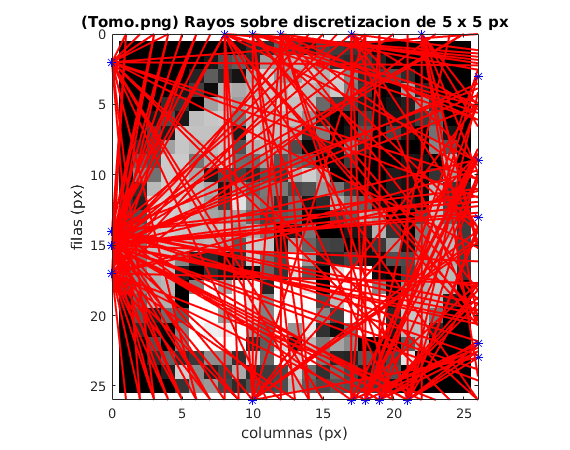
\includegraphics[width=1\textwidth]{img/rayos_tomo25x25px.png}
%\caption{Trazado aleatorio de rayos}
%\label{fig:rayos aleatorios}
%\end{figure}



